% !TEX encoding = UTF-8
% !TEX TS-program = pdflatex
% !TEX root = ../tesi.tex

%**************************************************************
\chapter{Resoconto dello stage}
\label{cap:descrizione-stage}
%**************************************************************

%**************************************************************


\section{Studio preliminare}
In questa sezione sono descritte le principali attività svolte durante il periodo di formazione preliminare. Tale periodo è stato di fondamentale importanza per permettermi un buon grado di autonomia durante lo svolgimento di tutta l'attività di stage.
\subsection{\textit{Process mining}}
Prima essermi inoltrato all'interno del problema, è stato necessario un periodo di formazione che ha ricoperto la durata di due settimane, durante il quale ho appreso i principi cardine del \textit{process minig}, cercando di capire le sua dinamiche e la sua utilità all'interno di un contesto aziendale ben formato, per poter poi metterle in pratica durante la realizzazione del progetto. Tale periodo è stato caratterizzato dalla visione di videolezioni online, per spiegare l'argomento in generale, e da incontri programmati con il tutor in cui verificava il mio effettivo apprendimento. Inizialmente ho trovato qualche difficoltà durante lo studio di tali nozioni, essendo stato per me un argomento completamente nuovo; ma dopo aver compreso le sue meccaniche sono riuscito ad applicare in maniera completa i suoi principi durante tutte l'arco dello stage.
\begin{figure}[!h] 
	\centering 
	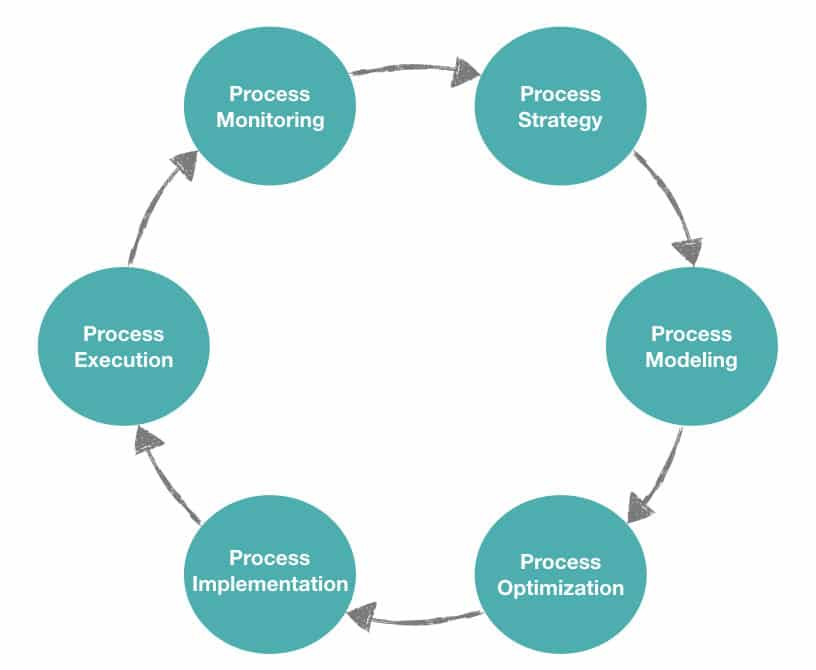
\includegraphics[width=0.8\columnwidth]{mining-lifecycle} 
	\caption{Ciclo di vita della gestione dei processi \url{https://lanalabs.com/en/what-is-process-mining-bpm/}}
\end{figure}

\subsection{Angular e \textit{typescript}}
In concomitanza con il periodo di formazine sopracitato sono stati svolti alcuni studi in merito al noto \textit{framework}, in modo da avere una buona base di partenza per poter procedere in autonomia allo sviluppo dell'interfaccia. Inizialmente, sotto consiglio del tutor, ho guardato la documentazione presente all'interno del sito di Angular, in modo da poter avere una panoramica generale. Successivamente sono sono stato affiancato per un breve periodo da diverse figure all'interno dell'azienda, sviluppando alcune interfacce basilari che poi mi sarebbero state utili al fine del prodotto finale, in modo da rendere più metodica ed immediata l'assimilazione delle principali strutture presenti in Angular;
\newpage
\section{Analisi dei requisiti}
Per poter tracciare i requisiti specifici necessari al compimento degli obiettivi, tramite consiglio del tutor, mi sono servito dei principali \textit{tool di process mining} presenti sul mercato, assieme al software interno all'azienda: \textit{Bipod}. In questo modo è stato possibile delineare una categorizzazione dei moduli di filtraggio richiesti, cercando di capire in che modo operassero nel concreto all'interno del log. Allo stesso modo sono stati tracciati ed analizzati i requisiti relativi all'interfaccia \textit{front-end}, confrontando le interfacce del loro applicativo con altri tool presenti in rete come \textit{ProM} e \textit{\gls{Disco}}. Per quanto riguarda lo \textit{stub} implementato è stato necessario uno studio preliminare dell'architettura finale, cercando di simularne il comportamento a seguito di richieste di filtraggi. 
\begin{figure}[!h] 
	\centering 
	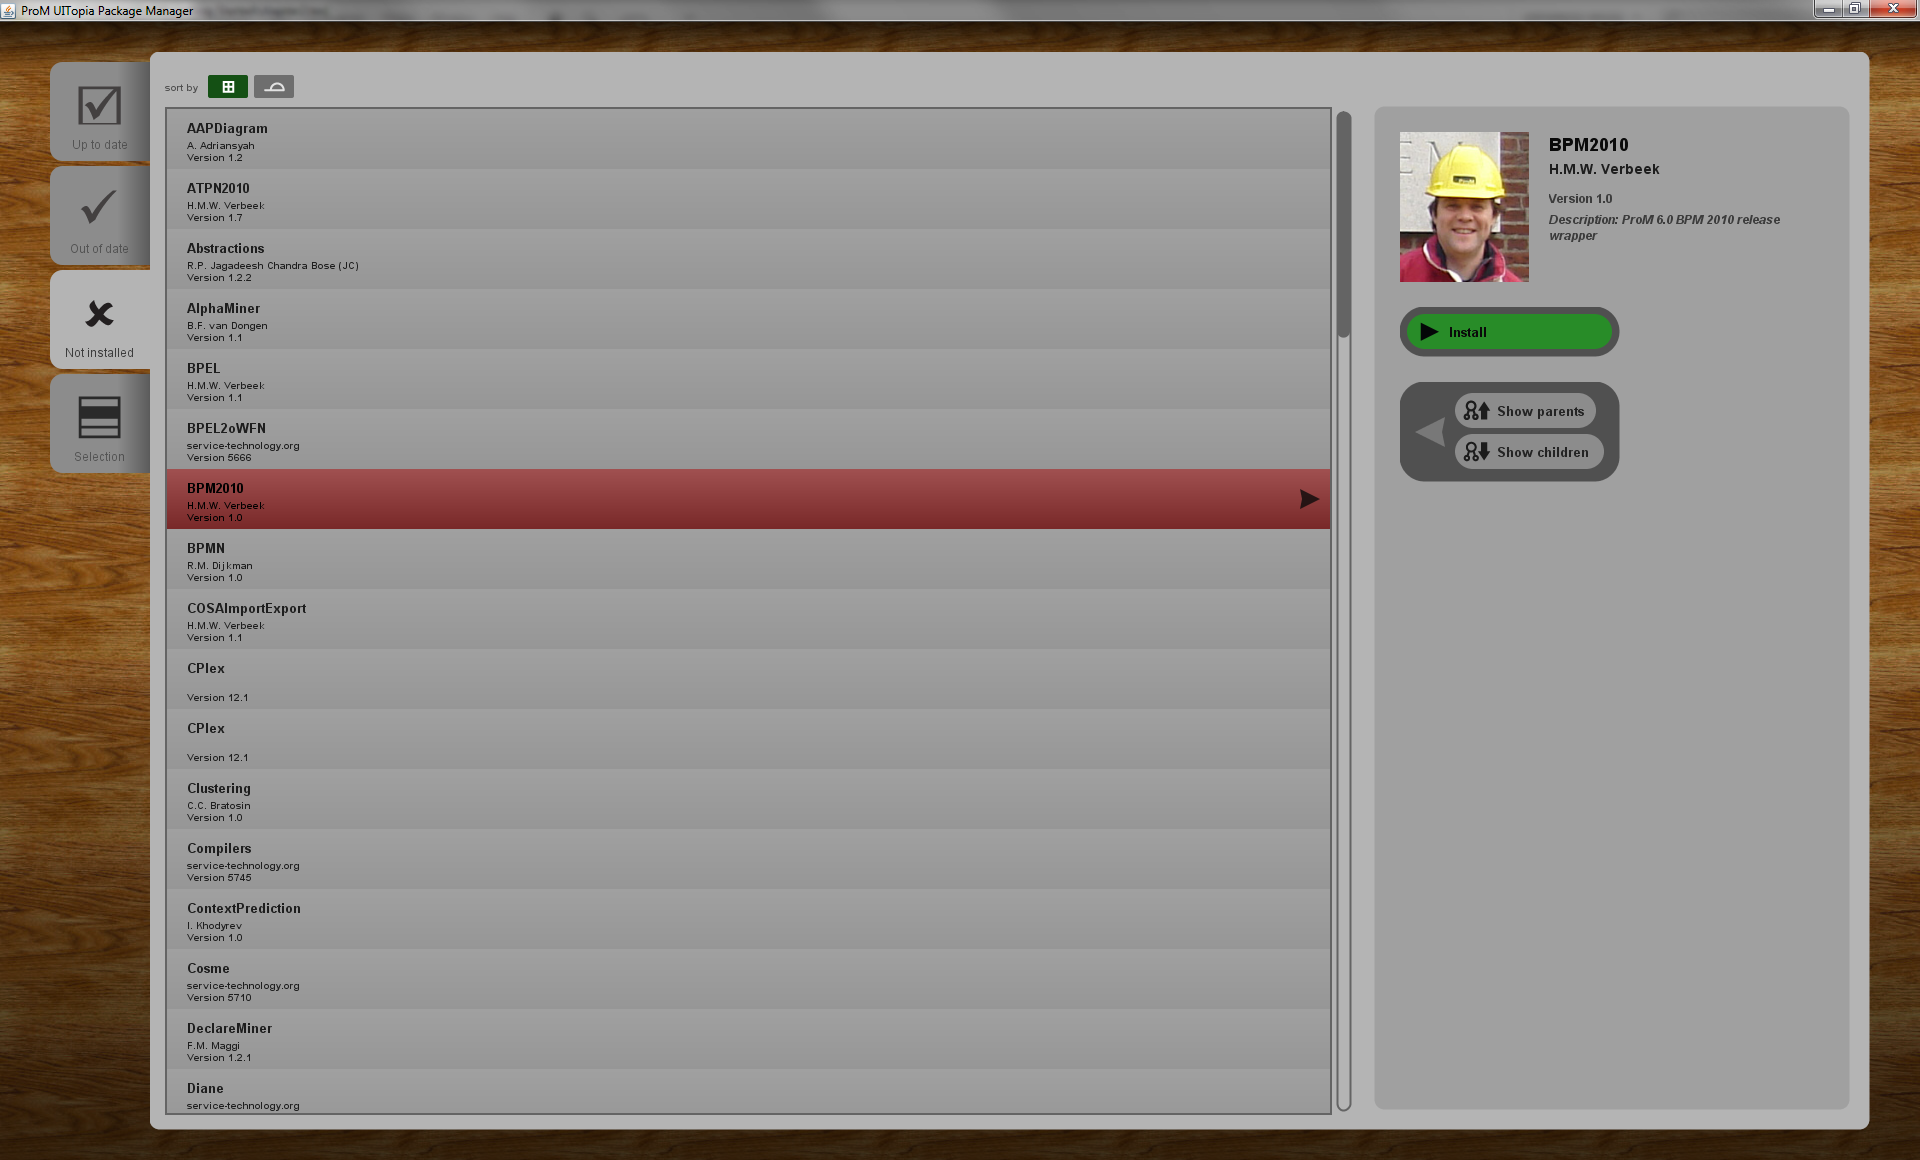
\includegraphics[width=0.8\columnwidth]{prom-package} 
	\caption{Package manager di ProM 6.x \url{http://www.promtools.org/doku.php?id=gettingstarted:installation}}
\end{figure}

\subsection{Libreria}
 Il \textit{tool} che mi ha permesso una maggior comprensione delle meccaniche di filtraggio, dandomi un buono spunto per l'implementazione della libreria è stato senz'altro \textit{ProM}; data la sua struttura modulare, a cui è possibile aggiungere esensioni di vario tipo, mi è stato possibile analizzarlo a fondo tramite lo studio del proprio repository. Mentre tramite gli altri \textit{tool} sono stato in grado di capire le dinamiche di filtraggio, tramite il repository di \textit{ProM} ho trovato alcuni esempi di implementazioni, anche se mal documentati e poco comprensibili; quest'ultimi sono però stati fondamentali per comprendere gli standard a cui far affidamento. Nel caso della libreria, lo standard adottato è stato \textit{OpenXES}. Quest'ultimo rappresenta la struttura del log in formato .xes, una struttura molto simile ai file di tipo \textit{xml}. \textit{OpenXES} descrive il log degli eventi tramite una struttura dati chiamata XLog. A partire da questa struttura è possibile modellare i dati in arrivo a proprio piacimento gestendoli come vere e proprie liste di eventi. Tali eventi, rappresentati dalla classe XEvent, contengono un serie di attributi che vanno a caratterizzare l'evento e ne permettono il loro reperimento. I principali requisiti che sono emersi da questa analisi riguardano la categorizzazione delle tipologie di filtraggio, la loro implementazione ed il loro scopo. Sono state quindi delineate le seguenti tipologie:
\begin{itemize}
	\item Filtraggio basato su valori di \textit{timestamp}
	\item Filtraggio basato sulle performance degli eventi.
	\item Filtraggio basato su eventi consecutivi
	\item Filtraggio basato sugli attributi
	\item Filtraggio basato sulle varianti
	\item Filtraggio basato su \textit{endpoint}
\end{itemize}
\begin{figure}[!h] 
	\centering 
	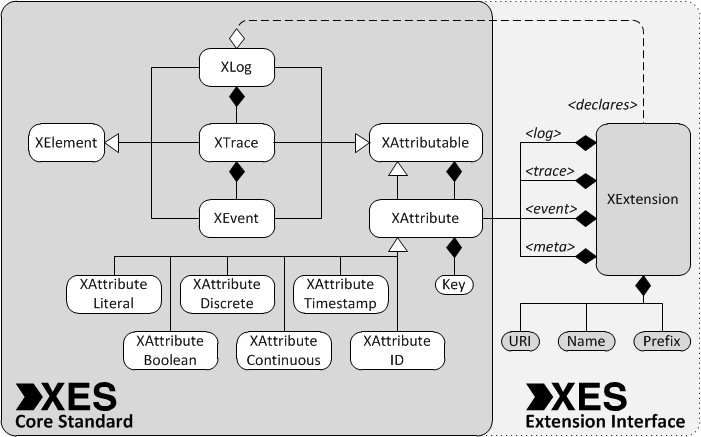
\includegraphics[width=1.0\columnwidth]{openxes} 
	\caption{Diagramma dei package dello standard OpenXes (\url{http://www.xes-standard.org/openxes/start})}
\end{figure}
Oltre alle funzionalità di filtraggio la libreria dovrebbe includere una serie di metodi legati al rilevamento di alcune caratteristiche del log in forma generica, in modo da poter determinare a priori alcune caratteristiche generali per poi agire di conseguenza.
Tali funzionalità di categorizzazione sono state pensate per favorire l'adattamento dell'interfaccia \textit{front-end} a fronte alle diverse tipologie di log che potevano venir esaminate dall'utente.
\subsection{\textit{Front-end}}
Per quanto rigurda i requisiti lato \textit{front-end} mi sono basato innanzitutto sullo studio dell'attuale \textit{tool} presente in azienda, cercando di inquadrare in modo chiaro tutte le interfacce atte allo svolgimento di operazioni di filtraggio. Dopo aver effettuato questa analisi, ho discusso a fondo con il tutor in merito ad una specifica interfaccia: quella riguardante il filtraggio sulle performance. Il vecchio applicativo presentava un'interfaccia poco intuitiva in cui non era ben chiaro nè la sua utilità, nè le sue funzionalità. È stato quindi deciso di riscrivere l'interfaccia cercando di semplificare la visualizzazione attuale, redendo più piacevole ed intuitiva l'esperienza utente. Inoltre è stato fortemente richiesto dal tutor che l'interfaccia risultasse scalabile ed adattabile in modo da poter estendere il suo utilizzo a qualsiasi tipo di \textit{device}. Il risultato finale sarebbe quindi stata un'interfaccia solida ed intuitiva introducendo il supporto per le comunicazioni tramite \textit{\gls{Websocket}} e la gestione dei messaggi in arrivo dal server. Sono state quindi fissate le interfacce per ogni tipologia di filtraggio presente all'interno della libreria.

\subsection{\textit{Stub}}
Dopo la fase di negoziazione dei requisiti con il tutor aziendale, è stato deciso in comune accordo che la parte riguardante l'architettura del \textit{back-end} venisse accantonata, dato il tempo limitato a mia dispoizione e la sua rilevante complessità. Questo per far spazio ad uno \textit{Stub} che andasse a simulare il comportamento dell'architettura finale a fronte di una richiesta di filtraggio per valori temporali. Tale \textit{Stub} avrebbe dovuto comunicare con il \textit{Client} tramite un canale \textit{Websocket}, andando a gestire tutte le tipologie di messaggi ritornati dal server.
\begin{figure}[!h] 
	\centering 
	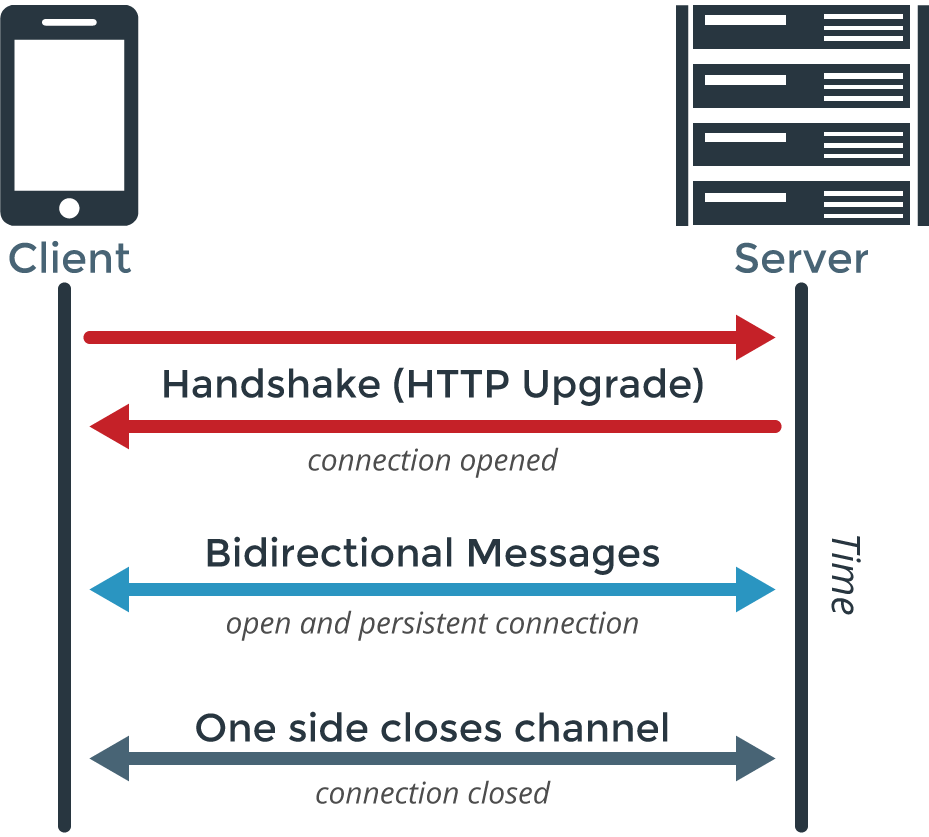
\includegraphics[width=0.6\columnwidth]{websocket} 
	\caption{Ciclo di vita di una connessione tramite websocket \url{https://radu-matei.com/blog/aspnet-core-websockets-middleware/}}
\end{figure}
\newpage
\section{Progettazione}
\subsection{Libreria}
Dopo aver delineato i principali requisiti da dover soddisfare sono passato alla fase di progettazione, cercando di strutturare la libreria in modo semplice, ma allo stesso tempo efficace, andando a documentare ogni singola funzionalità tramite \textit{\gls{Javadoc}}, in modo da rendere mantenibile l'intera libreria e soprattutto renderla comprensione ai futuri utilizzatori. È stato deciso di dividerla in più classi, ognuna di esse riguardante una tipologia di filtraggio, in modo da rendere la sua lettura più semplice ed immediata. Tutti i metodi presenti all'interno della libreria operano su tipi di dato in formato standard derivati da \textit{OpenXES}, questo è stato un requisito fortemente richiesto dal tutor interno. Oltre alle operazioni di filtraggio sono stati inclusi altri metodi per poter effettuare degli studi preliminare sul log preso in esame, andando a catalogarlo sotto determinati aspetti che, al fine di tutto l'applicativo, risultano di fondamentale importanza. Le principali classi che comporrano la libreria di filtraggio saranno dunque sei, ossia quelle che sono state delineate tramite analisi dei requisiti.
In aggiunta saranno presenti altre due classi che andranno a delineare i metodi di categorizzazione generale del log sulla base del \textit{lifecycle} e delle varianti. All'interno di ogni classe dovranno essere presenti dei metodi pubblici a cui l'utente avrà accesso diretto ed una parte di metodi privati che saranno invocati da quelli appena descritti ed andranno ad effettuare operazioni elementari sul log in modo da poter aderire al principio \textit{\gls{open-closed}}.
\subsection{\textit{Front-end}}
Per poter eseguire una fase di Progettazione trasparente rispetto ai requisiti analizzati mi sono avvalso di alcuni \textit{\gls{mockup}} tramite i quali, sotto la supervisione del tutor, mi hanno permesso di tracciare tutte le interfacce di filtraggio, andando a rispettare tutti i requisiti preposti. Tali modelli sono stati ideati allo stesso modo con cui è stata progettata la libreria: utilizzando un \textit{layout} a schede, dove, per ognuna di esse, è presente una tipologia di filtraggio. Un requisito che è stato fortmente richiesto da parte del tutor è stata la scalabilità dei componenti, andando ad inserire misure in percentuale ad ogni aspetto dell'interfaccia; Come per la fase di analisi dei requisiti anche in questo caso il filtraggio sulle performance ha richiesto una particolare attenzione: nel vecchio applicativo tale interfaccia era mal strutturata e non era ben chiaro all'utente che tipo di filtraggio stesse utilizzando. Ciò era dovuto ad un aspetto che prima d'ora non era stato preso in considerazione: il \textit{lifecycle} delle attività. Questo aspetto ha portato ad un lunga discussione con il tutor ed i membri del team in merito alle scelte da adottare. Ne è emerso che sarebbe stato necessario una differente interfaccia utente in base alla tipologie di \textit{lifecycle} presente all'interno del log. Tali metodi sono stati opportunamente implementati all'interno della libreria.\\
Per quanto rigurarda la futura interazione con i servizi \textit{back-end} è stato necessario avvalersi di \textit{RxJS}; una libreria sviluppata per \textit{javascript} che presenta tutte le principali funzionalità per la gestione dei messaggi tramite canali \textit{websocket}. Questa libreria è in grando di reperire i messaggi in arrivo tramite un gestore di \textit{callback} che differenzia i vari messaggi e fa reagire l'interfaccia in modo diverso a seconda della tipologia in arrivo. I messaggi vengono trasmessi all'interno del canale sottoforma di file \textit{\gls{JSON}}.
\begin{figure}[!h] 
	\centering 
	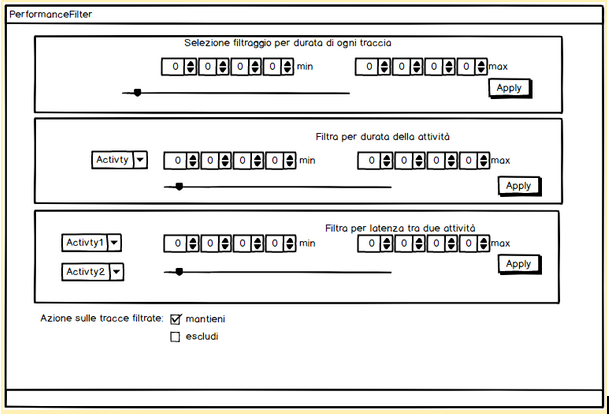
\includegraphics[width=0.9\columnwidth]{mockup} 
	\caption{Mockup ottenuto per l'interfaccia riguardante il filtraggio per performance}
\end{figure}
\subsection{\textit{Stub}}
Prima di poter passare alle realizzazione dello Stub è stato necessario dare una particolare attenzione all'architettura finale del \textit{back-end}. Purtroppo, date le strette tempistiche da rispettare e le varie criticità riscontrate durante le fasi precedenti è stato possibile comprenderla solamente a livello teorico. Tale architettura si basava quindi su un sistema a microservizi all'interno del quale erano presenti degli \textit{worker} che reagivano a determinate richieste lato \textit{client}. Nel momento in cui veniva presa in carico l'operazione, il \textit{worker} ritornava messaggi di progresso, indicando lo stato di avanzamento dell'operazione, che andavano quindi ad ag aggiornare l'interfaccia. Al momento della terminazione, il servizio inviava il relativo messaggio, che andava a notificare l'utente sull'effettivo completamento dell'operazione.\\


\begin{figure}[!h] 
	\centering 
	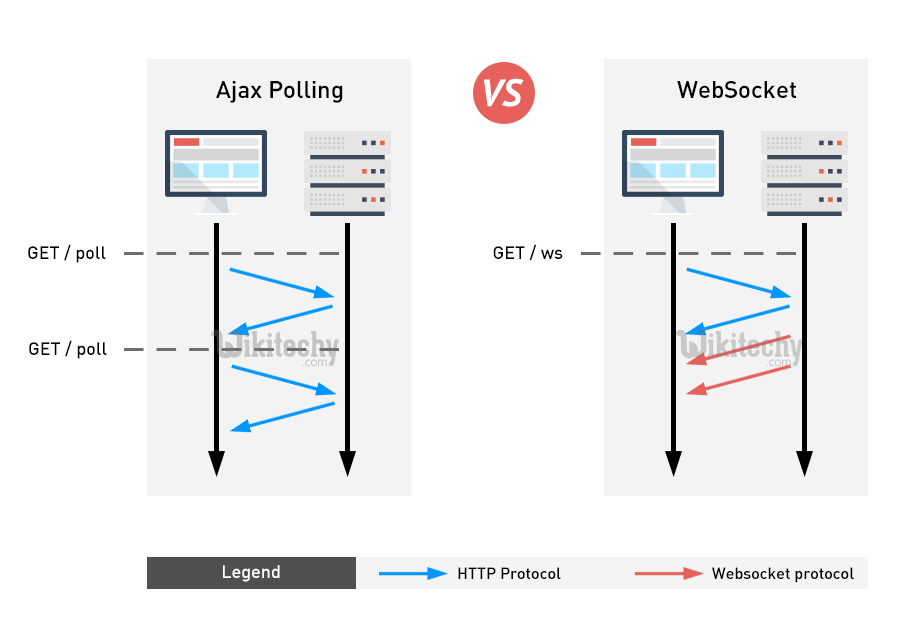
\includegraphics[width=0.9\columnwidth]{websocket-vs-ajax} 
	\caption{Differenza tra una chiamata websocket ed una http \url{https://www.wikitechy.com/tutorials/socket/differences-between-websockets-and-ajax}}
\end{figure}

\section{Codifica}
Avendo svolto una buona analisi dei requisiti seguiti da una solida progettazione, la  fase di codifica non ha portato a grosse criticità. Tale processo ha influito però su alcuni aspetti che non erano stati presi in considerazione prima d'ora.
\subsection{Libreria}
Per la codifica della libreria ho seguito in modo meticoloso i punti cardine fissati durante le fasi precedenti. Le principali criticità riscontrate riguardavano l'efficenza dei metodi. Un log degli eventi può rappresentare una struttura molto grande e complessa, a tal proposito non era ben chiaro se il log filtrato, ritornato dai vari metodi, dovesse essere una copia, creando di conseguenza una cospicua occupazione di memoria. Per far fronte a ciò è stato deciso di delegare tale scelta all'architettura del \textit{back-end}; andando a scegliere in base alla dimensione del log preso in esame quale fosse la scelta più performante. Il risultato ottenuto dopo tale processo è stata un libreria contente sette classi, categorizzate in base allo loro utilità. Sono stati implementati nel complessivo 22 metodi pubblici e 9 privati, ognuno di essi documentato secondo lo standard \textit{Javadoc}.
\subsection{\textit{Front-end}}
Per poter rendere l'interfaccia limpida e trasparente all'utente è stato necessario ricercare all'interno di varie librerie presenti sul web i componenti \textit{Angular} che si adattassero in maniera migliore rispetto alle aspettative. Ciò ha comportato ad un ingente investimento in termini di risorse, dovendo far fronte ad eventuali problematiche riscontrate dal funzionamento specifico di tali componenti. Questo ha portato ad una continua ricerca di componenti performanti, sia dal punto di vista grafico, in termini di scalabilità, sia dal punto di vista della gestione delle risorse.
Per quanto riguarda l'integrazione con le connessioni tramite \textit{websocket} è stato scelto di utilizzare una caratterizzazione univoca della richieste da inviare tramite questo canale: la struttura del messaggio ideata è stata implementata nella forma seguente:
\begin{figure}[!h] 
	\centering 
	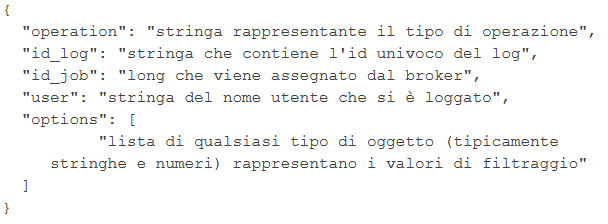
\includegraphics[width=0.8\columnwidth]{messaggiows} 
	\caption{Struttra della richiesta di filtraggio inviata al server tramite canale websocket}
\end{figure}
\subsection{Stub}
Lo stub non ha richiesto particolari criticità durante la sua fase di codifica, esso infatti è risultato un semplice file \textit{python} contenente i metodi di risposta da dover ritornare al \textit{front-end} a fronte di richieste di filtraggio. Tali messaggi dovevano poi essere intepretati dal \textit{client} per poi reagire di conseguenza. Per la struttura dei messaggi in uscita è stato scelto un formato univoco per qualsiasi tipologia in modo da uniformarne la ricezione anche lato \textit{front-end}.
\newpage
\section{Verifica e Validazione}
Sia la fase di verifica che quella di validazione è stata svolta in collaborazione con il tutor. Un fase di verifica veniva svolta, tipicamente, alla fine della settimana lavorativa, in cui venivano confrontate le attività preposte ad inizio settimana e confrontate con quelle realmente fatte, osservandone attentamente i punti fondamentamentale per verificare la presenza di errori o malfunzionamenti del sistema.\\ La fase di validazione è stata svolta durante l'ultima settimana di stage; in questa fase è stata confrontata la lista di tutte le varie attività svolte con i relativi obiettivi e requisiti concordati all'interno del piano di lavoro e rinegoziati durante il periodo successivo. Ciò ha portato alla conferma dell'effettiva terminazione delle attività in modo soddisfacente. 

\section{Risultati ragguinti}
La libreria è risultata ben formata in ogni sua parte, è stato fatto un buon lavoro di copertura del codice attraverso \textit{\gls{unit test}} mediante il quale sono stati testati 27 metodi dei 31 complessivi tra pubblici e privati; questo ha permesso di raggiungere una coprtura del 87\%. Ciò ha portato ad un buon grado di soddisfacimento sia da parte del tutor, sia a livello personale.\\
Lato \textit{front-end} sono state effettuate alcune prove strutturali dovute al ridimensionamento dell'interfaccia. In questo modo è stato possibile constatare che l'interfaccia fosse solida e ben formata. Purtroppo, a causa di alcune limitazioni dovute all'architettura del \textit{back-end} illustati nel capitoli precenti, non è stato possibile testare il suo effettivo funzionamento in ogni sua parte; pertanto mi sono concentrato esclusivamente in un'unica interfaccia di filtraggio, gestendo in maniera soddisfacente ogni suo comportamento a fronte di eventi che venivano ritornati dallo stub.\\
Nel complesso tutti i processi svolti hanno avuto uno scopo ben prciso per la realizzazione del prodotto finale. La libreria ha raggiunto un buon grado di affidabilità e mantenibilità in cui sarà possibile includere eventuali funzionalità aggiuntive in maniera diretta. Il \textit{front-end} è risultato molto solido a livello grafico, mantenendo la stessa struttura anche a fronte di ridimensionamti consistenti. L'integrazione delle chiamate \textit{websocket} e del relativo stub hanno mantenuto comunque l'interfaccia solida senza comportare alcun tipo di malfunzionamento. Ciò ha portato ad un significativo passo in avanti guardando nell'ottica dell'applicativo finale che dovrà rilasciare \textit{Siav}.